\section{Tìm cực trị của hàm số biết bảng biến thiên hoặc đồ thị}
\subsection{Kiến thức cần nhớ}
\begin{khung}
	Dựa vào bảng biến thiên hoặc đồ thị hàm số nhận biết việc đổi dấu của đạo hàm $f'(x)$ để kết luận
	\begin{itemize}
		\item Nếu $f'(x)$ đối dấu từ âm sang dương khi qua điểm $x_0$ thì $x_0$ là điểm cực tiểu của hàm số.
		\item Nếu $f'(x)$ đổi dấu từ dương sang âm khi qua điểm $x_0$ thì $x_0$ là điểm cực đại của hàm số.
	\end{itemize}
\end{khung}
\subsection{Bài tập mẫu}
\Opensolutionfile{ans}[ans/ANS-DANG-19]
\setcounter{vd}{18}
\begin{khung}
%Câu 1
\begin{vd}[Đề minh họa BGD 2022-2023]%[2D1B2-2]
	\immini{
		Cho hàm số $y=ax^4+bx^2+c$ có đồ thị là đường cong trong hình bên. Điểm cực tiểu của đồ thị hàm số đã cho có tọa độ là
		\choice
		{$(-1;2)$}
		{\True $(0;1)$}
		{$(1;2)$}
		{$(1;0)$}
	}{
		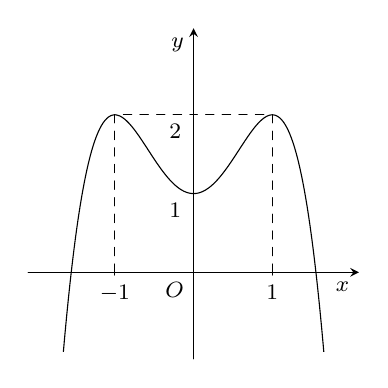
\begin{tikzpicture}[scale=1, font=\footnotesize, line join=round, line cap=round, >=stealth]
			\draw[->] (-2.1,0)--(2.1,0) node[below left] {$x$};
			\draw[->] (0,-1.1)--(0,3.1) node[below left] {$y$};
			\draw (0,0) node [below left] {$O$};
			\foreach \x in {-1,1}
			\draw[thin] (\x,1pt)--(\x,-1pt) node [below] {$\x$};
			\foreach \y in {1,2}
			\draw[thin] (1pt,\y)--(-1pt,\y) node [below left] {$\y$};
			\draw[dashed,thin](-1,0)--(-1,2)--(0,2);
			\draw[dashed,thin](1,0)--(1,2)--(0,2);
			\begin{scope}
				\clip (-2,-1) rectangle (2,3);
				\draw[samples=200,domain=-1.7:1.7,smooth,variable=\x] plot (\x,{-(\x)^4+2*(\x)^2+1});
			\end{scope}
		\end{tikzpicture}
	}
	\loigiai{
		Quan sát đồ thị ta thấy điểm cực tiểu của đồ thị hàm số đã cho có toạ độ là $(0;1)$.
	}
\end{vd}
\end{khung}
\subsection{Bài tập tương tự và phát triển}
%Câu 2
\begin{ex}%[2D1B2-2]
\immini{
	Cho hàm số $y=f(x)$ xác định trong khoảng $(a,b)$ và có đồ thị như hình bên dưới. Trong các khẳng định dưới đây, khẳng định nào \textbf{sai}?
\choice
{Hàm số $y=f(x)$ có đạo hàm trong khoảng $(a;b)$}
{\True $f'(x_2) >0$}
{$f'(x_3) =0$}
{$f'(x_1) >0$}	
}{
	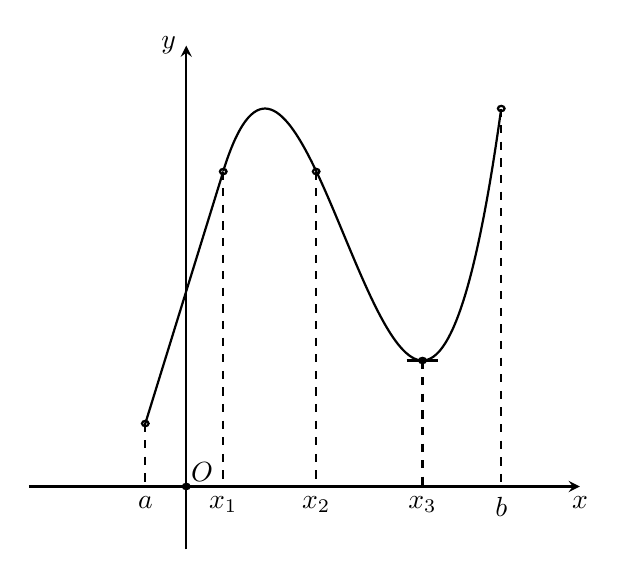
\begin{tikzpicture}[>= stealth,thick,yscale=.8]
	\coordinate (A) at (0.47,5) ;
	\coordinate (B) at (-0.52,1);
	\coordinate (C) at (3,2);
	\coordinate (D) at (1.65,5);
	\coordinate (E) at (4,6);
	\draw[->] (-2,0)--(5,0) node[below] {$x$};
	\draw[->] (0,-1)--(0,7) node[left] {$y$};
	\draw[fill=black] (0,0) circle (1.2pt) node[above right=-2pt] {$O$};
	\draw (A)--(B);
	\draw (2.8,2)--(3.2,2);
	\draw[dashed] (B)--(-0.52,0) node[below] {$a$};
	\draw[dashed] (A)--(0.47,0) node[below] {$x_1$};
	\draw[dashed] (D)--(1.65,0) node[below] {$x_2$};
	\draw[dashed] (C)--(3,0) node[below] {$x_3$};
	\draw[dashed] (E)--(4,0) node[below] {$b$};
	\foreach \i in {A,B,C,D,E} \draw (\i) circle (1.2pt);
	\draw[smooth,samples=100, domain=0.47:4] plot(\x,{((\x)-1.0)^(3.0)-3.0*((\x)-1.0)^(2.0)+6.0});
\end{tikzpicture}
}
	\loigiai{
	Dựa vào đồ thị ta thấy hàm số có đạo hàm và nghịch biến trong khoảng $(c;d)$ chứa $x_2$, suy ra $f'(x_2) \leq 0$.
}
\end{ex}

%Câu 3
\begin{ex}%[2D1Y2-2]
	Cho hàm số $y=f(x)$ có bảng biến thiên như sau
	\begin{center}
		
\begin{tikzpicture}
			\tkzTabInit[nocadre=false,lgt=1.2,espcl=2.5,deltacl=0.6]
			{$x$ /0.6,$y'$ /0.6,$y$ /2}
			{$-\infty$,$-2$,$0$,$2$,$+\infty$}
			\tkzTabLine{,-,$0$,+,$0$,-,$0$,+,}
			\tkzTabVar{+/$+\infty$, -/$0$,+/$3$,-/$0$,+/$+\infty$}
		\end{tikzpicture}
	\end{center}
	Chọn khẳng định \textbf{sai}.
	\choice
	{$f(x)\geq0$, $\forall x\in\mathbb{R}$}
	{Hàm số $f(x)$ đồng biến trên $(3;+\infty)$}
	{\True Hàm số $f(x)$ đạt cực đại tại $x=3$}
	{Hàm số $f(x)$ nghịch biến trên $(-\infty;-3)$}
	\loigiai{
		Dựa vào bảng biến thiên, ta thấy hàm số $f'(x)$ tại điểm $x=3$ không đổi dấu nên $f(x)$ không đạt cực trị tại $x=3$.
	}
\end{ex}

%Câu 4
\begin{ex}%[2D1Y2-2]
	Cho hàm số $ y=f(x) $ liên tục trên $ \mathbb{R} $ và có bảng xét dấu của đạo hàm như hình vẽ. 
	\begin{center}
		
\begin{tikzpicture}[scale=0.7, font=\footnotesize, line join=round, line cap=round, >=stealth]
			\tkzTabInit[nocadre=false,lgt=2,espcl=2,deltacl=0.5]{$x$/1 ,$f'(x)$/1}
			{$-\infty$ , $-1$ , $0$ , $2$,$ 4$, $+\infty$}
			\tkzTabLine{  , + , $ 0 $ , - , d , + ,$ 0 $, -,$ 0 $ ,+, }
		\end{tikzpicture}
	\end{center}
	Hàm số đã cho có
	bao nhiêu điểm cực trị?
	\choice
	{$ 2 $}
	{$ 1 $}
	{$ 3 $}
	{\True$ 4 $}
	\loigiai{
		Ta thấy $ f'(x) $ đổi dấu $ 4 $ lần, và $ f(x) $ liên tục trên $ \mathbb{R} $, suy ra hàm số có $ 4 $ điểm cực trị.}
\end{ex}

%Câu 5
\begin{ex}%[2D1Y2-2]
	Cho hàm số $y=f(x)$ liên tục trên $\mathbb{R}$ và có bảng biến thiên như bảng sau.
	\begin{center}
		
\begin{tikzpicture} [scale=.8]
			\tkzTabInit[lgt=1, espcl=2, deltacl=.6 ] {$x$ /.7, $y'$/.7, $y$/2 }%
			{$-\infty$,$-3$,$-2$,$3$,$+\infty$}%
			\tkzTabLine { ,-,d,+,0,-,d,+, }
			\tkzTabVar{+/$+\infty$ ,-/$21$ ,+/$22$,-/$-3$,+/$+\infty$}
		\end{tikzpicture}
	\end{center}
	Tổng các giá trị cực tiểu của hàm số trên bằng
	\choice
	{$19$}
	{\True $18$}
	{$0$}
	{$22$}
	\loigiai{
		Tổng các giá trị cực tiểu của hàm số là $21-3=18$.}
\end{ex}

%Câu 6
\begin{ex}%[2D1B2-2]
	\immini{
		Cho hàm số $y=f(x)$ liên tục trên đoạn $[-4;3]$ và có đồ thị trên đoạn $[-4;3]$ như hình bên. Hãy xác định số điểm cực đại của đồ thị hàm số đó.
		\motcot
		{$3$}
		{$0$}
		{$2$}
		{\True $1$}
	}{
		\hspace{0.5cm}
		\begin{tikzpicture}[scale=0.8,>=stealth]
			\draw[->](0,-1)--(0,6)node[left]{$y$};
			\foreach \y in {1,2,5}
			\draw[yshift=\y cm,thick](-2pt,0pt)--(2pt,0pt)node[left,xshift=-2pt]{$\y$};
			\draw[->](-5,0)--(4,0)node[above]{$x$};
			\foreach \x in {-4,...,-1,1,2,3}
			\draw[xshift=\x cm,thick](0pt,-2pt)--(0pt,2pt)node[below,yshift=-2pt]{$\x$};
			\draw(0,0)node[below left]{$O$};
			\draw[smooth,samples=200,domain=-3:0]plot(\x,{(\x)^2+4*\x+5});
			\draw(-4,0)--(-3,2) (0,5)--(1,5)--(3,-1);
			\draw[fill=black](3,-1)circle(1pt);
			\draw[fill=black](-4,0)circle(1pt);
		\end{tikzpicture}
		\hspace{0.5cm}
	}
	\loigiai{
		Từ đồ thị bài cho ta thấy $y'$ đổi dấu từ dương sang âm tại $x=-3$ nên hàm số đạt cực đại tại đó. Vậy hàm số có một cực đại.
	}
\end{ex}

%Câu 7
\begin{ex}%[2D1B2-2]
	Cho hàm số $y=ax^3+bx^2+cx+d$, với $a$, $b$, $c$, $d$ là các số
	\immini{thực và $a\neq 0$, có đồ thị như hình bên. Khẳng định nào sau đây \textbf{sai}?\choice
		{$y'<0,\ \forall x\in(-2;0)$}
		{\True Hàm số đạt giá trị lớn nhất tại điểm $x=-2$}
		{Đồ thị hàm số có đúng hai điểm cực trị}
		{$f'(x)=0\Leftrightarrow\hoac{& x=-2\\ & x=0}$}
	}{
		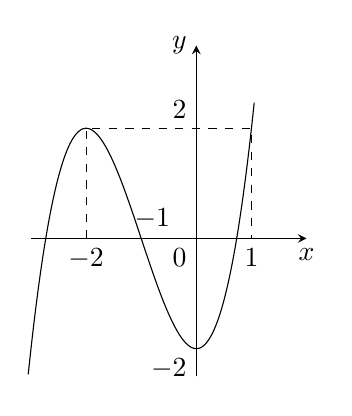
\begin{tikzpicture}[>=stealth,scale=0.7]
			\draw[->] (-3,0) -- (2,0) node[below] {$x$};
			\draw[->] (0,-2.5) -- (0,3.5) node[left] {$y$};
			\draw[smooth,samples=100,domain=-3.05:1.05] plot(\x,{(\x)^3+3*(\x)^2-2});
			\draw[dashed] (-2,0) node[below] {$-2$}--(-2,2)--(0,2)node[above left] {$2$}--(1,2)--(1,0) node[below] {$1$};
			\node[below left] at (0,-2) {$-2$};
			\node[above] at (-0.8,0) {$-1$};
			\node[below left] at (0,0) {$0$};
		\end{tikzpicture}
	}
	\loigiai{
		Khẳng định \textbf{sai} là: ``Hàm số đạt giá trị lớn nhất tại điểm $x=-2$''. Lí do: có thể thấy với $x>1$ thì $f(x)>f(-2)$.\\
		Sửa lại đúng: ``Hàm số đạt cực đại tại điểm $x=-2$''.
	}
\end{ex}

%Câu 8
\begin{ex}%[2D1Y2-2]
	\immini{Cho hàm số bậc bốn $y=f(x)$ liên tục trên $\mathbb{R}$ và có đồ thị là đường cong như hình vẽ bên. Tìm điểm cực tiểu của đồ thị hàm số $y=f(x)$.
		\choicew{.6\textwidth}
		\choice
		{$x=0$}
		{$y=-2$}
		{\True $M(0;-2)$}
		{$N(2;2)$}
	}{
		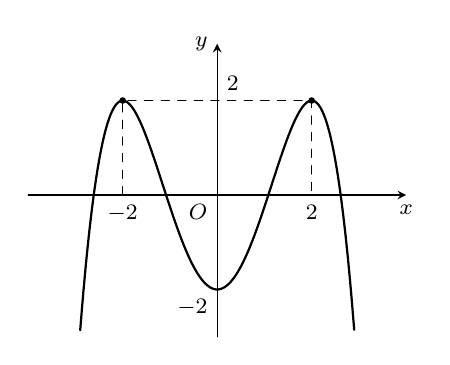
\begin{tikzpicture}[>=stealth, line cap=round, line join=round, font=\footnotesize,scale=.6]
			\draw[->] (-4,0)--(4,0)node[below]{$x$};
			\draw[->] (0,-3)--(0,3.2)node[left]{$y$};
			\draw[thick,smooth,samples=100,domain=-2.9:2.9] plot(\x,{-(\x)^4/4+2*(\x)^2-2});
			\draw (-2,0)node[below]{$-2$} (2,0)node[below]{$2$} (0,-2)node[below left]{$-2$} (0,2)node[above right]{$2$} (0,0)node[below left]{$O$};
			\draw[dashed] (-2,0)--(-2,2)--(2,2)--(2,0);
			\fill (-2,2)circle(2pt) (2,2)circle(2pt);
	\end{tikzpicture}}
	\loigiai{
		Điểm cực tiểu của đồ thị hàm số là $M(0;-2)$.
	}
\end{ex}

%Câu 9
\begin{ex}%%[2D1B2-2]
Cho hàm số $y=f\left(x\right)$ liên tục trên từng khoảng xác định và có bảng biến thiên như sau.
\begin{center}
	
\begin{tikzpicture}[>=stealth]
		\tkzTabInit[nocadre=false,lgt=1,espcl=2,deltacl=0.5]{$x$/.7 ,$y'$/.7,$y$/2}
		{$-\infty$ , $x_1$,$x_2$ , $+\infty$}
		\tkzTabLine{ , + , d ,-,d, + , }
		\tkzTabVar{-/$-\infty$ ,+D+/$+\infty$/$+\infty$ ,-/$0$, +/$+\infty$}
	\end{tikzpicture}
\end{center}
 Khẳng định nào sau đây \textbf{đúng}?
		\choice
		{Hàm số đã cho không có cực trị}
		{\True Hàm số đã cho có một điểm cực tiểu và không có điểm cực đại}
		{Hàm số đã cho có một điểm cực đại và có một điểm cực tiểu}
		{Hàm số đã cho có một điểm cực đại và không có điểm cực tiểu}

	\loigiai{
		Hàm số không xác định tại $x_1$ nên $x_1$ không là điểm cực trị.\\
		Tại $x_2$ hàm số không có đạo hàm nhưng vẫn xác định, đồng thời đạo hàm đổi dấu khi qua $x_2$ nên $x_2$ là điểm cực tiểu.
	}
\end{ex}

%Câu 10
\begin{ex}%[2D1Y2-2]
	Cho hàm số $y=f(x)$ liên tục trên $(-\infty;4]$ và có bảng biến thiên như hình vẽ sau
	\begin{center}
		
\begin{tikzpicture}
			\tkzTabInit[nocadre=false,lgt=1.2,espcl=2.5,deltacl=0.6]
			{$x$ /0.6,$y'$ /0.6,$y$ /2}
			{$-\infty$,$1$,$2$,$3$,$4$}
			\tkzTabLine{,+,$0$,-,d,+,$0$,-,}
			\tkzTabVar{-/$-\infty$, +/$1$,-/$0$,+/$2$,-/$-1$}
		\end{tikzpicture}
	\end{center}
	Số điểm cực trị của hàm số đã cho là
	\choice
	{$4$}
	{\True $3$}
	{$2$}
	{$5$}
	\loigiai{
		Dựa vào bảng biến thiên, ta thấy hàm số đã cho có $3$ điểm cực trị.
	}
\end{ex}

%Câu 11
\begin{ex}%[2D1B2-2]
	Cho hàm số $y=f(x)$ liên tục trên $\mathbb{R}$ và có bảng biến thiên như sau. 
	\begin{center}
		
\begin{tikzpicture}
			\tkzTab
			[lgt=2,espcl=2.5]
			{$x$/1, $f’(x)$/1, $f(x)$/2.5}
			{$-\infty$, $-1$, $0$, $1$, $+\infty$}
			{,+,0,-,d,+,0,-,}
			{-/ $-\infty$, +/ $4$, -/ $3$, +/ $4$ , -/ $-\infty$}
		\end{tikzpicture}
	\end{center}
Khẳng định nào dưới đây \textbf{sai}?
	\choice
	{Hàm số có ba điểm cực trị}
	{Hàm số đạt cực tiểu tại điểm $x=0$}
	{\True Hàm số có giá trị cực tiểu bằng $0$}
	{Hàm số có giá trị cực tiểu bằng $3$}
	\loigiai{
		Dựa vào bảng biến thiên ta thấy
		\begin{itemize}
			\item Hàm số đạt cực đại tại $x=\pm 1$. Giá trị cực đại $y=4$.
			\item Hàm số đạt cực tiểu tại $x=0$. Giá trị cực tiểu là $y=3$.
		\end{itemize}
	}
\end{ex}
%Câu 12
\begin{ex}%[2D1B2-2]
	Cho hàm số $y=f(x)$ liên tục trên $\mathbb{R}$ và có bảng xét dấu của $f'(x)$ như sau
	\begin{center}
		
\begin{tikzpicture}
			\tkzTabInit[nocadre=false,lgt=1.2,espcl=2.5,deltacl=0.6]
			{$x$ /0.6,$f'(x)$ /0.6}
			{$-\infty$,$-2$,$1$,$5$,$+\infty$}
			\tkzTabLine{,+,d,-,$0$,-,$0$,+,}
		\end{tikzpicture}
	\end{center}
	Số điểm cực trị của hàm số $y=f(x)$ là
	\choice
	{$3$}
	{\True $2$}
	{$0$}
	{$1$}
	\loigiai{
		Dựa vào bảng xét dấu của $f'(x)$ ta thấy $f'(x)$ đổi dấu hai lần.\\
		Vậy số điểm cực trị của hàm số là $2$.
	}
\end{ex}
%Câu 13
\begin{ex}%[2D1B2-2]
	\immini{ Cho hàm số $y=f(x)$ có đạo hàm trên $\mathbb{R}$. Biết rằng hàm số $y=f'(x)$ có đồ thị như hình bên.
		Đặt $g(x)=f(x)+x.$ Hỏi hàm số có bao nhiêu điểm cực đại và bao nhiêu điểm cực tiểu trên khoảng $(-1;3)$?
		\choice
		{Hàm số có một điểm cực đại và hai điểm cực tiểu}
		{Hàm số có một điểm cực đại và một điểm cực tiểu}
		{Hàm số không có điểm cực đại và có một điểm cực tiểu}
		{\True Hàm số có hai điểm cực đại và một điểm cực tiểu}
	}
	{        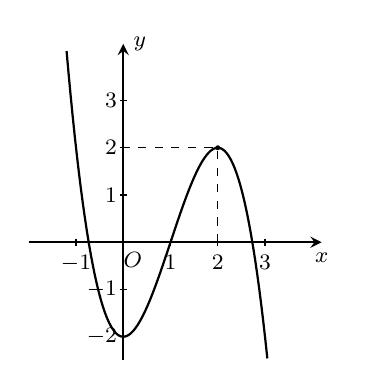
\begin{tikzpicture}[>=stealth,font=\footnotesize,scale=0.6]
%			\draw[dashed,thin,gray] (-2.5,-2.5) grid[step=0.5] (4.5,4.5);
			\draw[thick,->] (-2,0)--(4.2,0) node[below]{$x$};
			\draw[thick,->] (0,-2.5)--(0,4.2) node[right]{$y$};
			\draw (-0.2,0)node[below right]{$O$};
			\draw[thick,color=black,samples=100,domain=-1.2:3.05] plot (\x,{-(\x)^3+3*(\x)^2-2});
			\foreach \x in {-1,1,2,3}
			\draw[shift={(\x,0)}] (0,2pt)--(0,-2pt) node[below]{$\x$};
			\foreach \y in {-2,-1,1,2,3}
			\draw[shift={(0,\y)}] (-2pt,0)--(2pt,0) node[left]{$\y$};
			\fill (2,2)circle(1.5pt);
			\draw[dashed] (2,0)--(2,2)--(0,2);
		\end{tikzpicture}
	}
	\loigiai{
		Hàm số $f(x)$ có đạo hàm trên $\mathbb{R}$ nên hàm số $g(x)=f(x)+x$ cũng có đạo hàm trên $\mathbb{R}$ và $g'(x)=f'(x)+1;g'(x)=0 \Leftrightarrow f'(x)=-1$.\\
		Dựa vào đồ thị $f^{'}(x)$ ta có $f^{'}(x)=-1$ có ba nghiệm phân biệt $x_1,x_2,x_3$ với $x_1<x_2<x_3$.\\
		Bảng biến thiên của $g(x)$:
		\begin{center}
			\begin{tikzpicture}
				\tkzTabInit[nocadre=false,lgt=1.5,espcl=2]
				{$x$ /1,$g'(x)$ /1,$g(x)$ /2}{$-1$,$x_1$,$x_2$,$x_3$,$3$}
				\tkzTabLine{,+,$0$,-,$0$,+,$0$,-,}
				\tkzTabVar{-/ $g(-1)$ ,+/$g(x_1)$,-/$g(x_2)$,+/$g(x_3)$,-/$g(3)$}
			\end{tikzpicture}
		\end{center}
		Hàm số có hai điểm cực đại và một điểm cực tiểu.}
\end{ex}
%Câu 14
\begin{ex}%[2D1K2-2]
	Cho hàm số bậc ba $y=f(x)$ có bảng biến thiên như hình vẽ.\\
	\begin{center}
		\begin{tikzpicture}[>=stealth,line join=round,line cap=round,font=\footnotesize,xscale=.8]
			\tikzset{
				declare function={
					step=-1;wide=\textwidth;hight=-5;length=wide-1;cstep=1.5;
				}
			}
			\begin{scope}[xshift=-0.5 cm,yshift=.5 cm]
				\draw (0,0) rectangle (wide,hight);
				\draw
				(0,step)--(wide,step)
				(0,step*2)--(wide,step*2)
				(1,0)--(1,hight)
				;
			\end{scope}
			\path
			%row-1
			(0,0)coordinate (A0)node{$x$}+(0:cstep)node{$-\infty$}coordinate (A1)+(0:wide-1cm)coordinate (An)node{$+\infty$}
			($(A1)!1/3!(An)$)node{$0$}
			($(A1)!2/3!(An)$)node{$2$}
			%row-2
			(0,step)coordinate (B1)node{$y'$}+(0:cstep)coordinate (B1)+(0:wide-1cm)coordinate (Bn)
			($(B1)!1/6!(Bn)$)node{$-$}
			($(B1)!2/6!(Bn)$)coordinate (B2)node{$0$}
			($(B1)!3/6!(Bn)$)node{$+$}
			($(B1)!4/6!(Bn)$)coordinate (B3)node{$0$}
			($(B1)!5/6!(Bn)$)node{$-$}
			%row-3
			(0,step*3)coordinate (C0)node{$y$}
			($(B1)+(90:step)$)coordinate (C1)node[fill=white]{$+\infty$}
			($(B2)+(90:step*3)$)coordinate (C2)node[fill=white]{$-3$}
			($(B3)+(90:step)$)coordinate (C3)node{$1$}
			($(Bn)+(90:step*3)$)coordinate (Cn)node{$-\infty$}
			;
			\foreach \pointo/\pointt in {C1/C2,C2/C3,C3/Cn}{
				\draw[fill=black,->,shorten <=.5cm,shorten >=.5cm](\pointo)--(\pointt);
			}
		\end{tikzpicture}
	\end{center}
	Hàm số $y=f\left(f(x)\right)$ có bao nhiêu điểm cực trị?
	\choice
	{$5$}
	{\True $6$}
	{$4$}
	{$7$}
	\loigiai{
		Ta có $y=f\left(f(x)\right)\Rightarrow{y}'=f'\left(f(x)\right)\cdot f'(x)$.\\
		Nên $y'=0\Leftrightarrow\left[\begin{aligned}
			&{f}'\left(f(x)\right)=0\\
			&{f}'(x)=0.\\
		\end{aligned}\right.$\\
		$f'(x)=0\Leftrightarrow x=0\vee x=2$.\\
		$f'\left(f(x)\right)=0\Leftrightarrow\left[\begin{aligned}
			& f(x)=0\qquad(1)\\
			& f(x)=2.\qquad(2)\\
		\end{aligned}\right.$ \\
		Phương trình $(1)$ cho chúng ta $3$ nghiệm phân biệt, $(2)$ cho chúng ta $1$ nghiệm và không trùng với nghiệm $x=0,x=2$ nên $y=f\left(f(x)\right)$ có $6$ điểm cực trị.
	}
\end{ex}

%Câu 15
\begin{ex}%[2D1K2-2]
	Cho hàm số $y=f(x)$ xác định và liên tục trên $\mathbb{R}$ và có đạo hàm\break $f'(x)=x^3(x+1)^2(2-x)$. Hàm số đã cho có bao nhiêu điểm cực trị?
	\choice
	{ $3$}
	{\True $2$}
	{ $0$}
	{$1$ }
	\loigiai{
		Ta có $f'(x)=0$ có ba nghiệm $x=0$, $x=-1$, $x=2$. Trong đó $x=0$ là nghiệm bội 3, $x=-1$ là nghiệm kép, $x=2$ là nghiệm đơn nên hàm số $y=f(x)$ có hai điểm cực trị là $x=0$ và $x=2$.
	}
\end{ex}
%Câu 16
\begin{ex}%[2D1K2-2]
	Cho hàm số $y=f(x)$ có đạo hàm trên $\mathbb{R}$ và có bảng biến thiên như hình vẽ sau
	\begin{center}
		
\begin{tikzpicture}[scale=1,font=\footnotesize,line join=round,line cap=round,>=stealth]
			\tkzTabInit[nocadre=false,lgt=1.2,espcl=2.5,deltacl=0.6]
			{$x$/0.8,$f(x)$/2}
			{$-\infty$,$-1$,$0$,$2$,+$\infty$}
			\tkzTabVar{-/$-\infty$,+/$1$,-/$-2$,+/$1$,-/$-\infty$}
		\end{tikzpicture}
	\end{center}
	Hàm số $y=f(2x)$ đạt cực đại tại điểm nào dưới đây?
	\choice
	{$x=\dfrac{1}{2}$}
	{$x=-2$}
	{\True $x=1$}
	{$x=-1$}
	\loigiai{
		Dựa vào bảng biến thiên, ta suy ra bảng xét dấu đạo hàm của hàm số $y=f(x)$ như sau:
		\begin{center}
			
\begin{tikzpicture}[scale=1, font=\footnotesize, line join=round, line cap=round, >=stealth]
				\tkzTabInit[nocadre=false,lgt=1.2,espcl=1.5,deltacl=0.6]
				{$x$/.7,$f'(x)$/.7}
				{$-\infty$,$-1$,$0$,$2$,$+\infty$}
				\tkzTabLine{,+,z,-,z,+,z,-,}
			\end{tikzpicture}
		\end{center}
		Xét hàm số $y=f(2x)$, ta có $y'=2\cdot f'(2x)$.\\
		Ta suy ra
		$$f'(x)=0\Leftrightarrow 2\cdot f'(2x)=0\Leftrightarrow \hoac{&2x=-1\\&2x=0\\&2x=2}\Leftrightarrow \hoac{&x=-\dfrac{1}{2}\\&x=0\\&x=1.}$$
		Bảng xét dấu của $y'=2\cdot f'(2x)$ là
		\begin{center}
			\begin{tikzpicture}[scale=1, font=\footnotesize, line join=round, line cap=round, >=stealth]
				\tkzTabInit[nocadre=false,lgt=2,espcl=2.5,deltacl=0.6]
				{$x$/0.6,$2f'(2x)$/0.6}
				{$-\infty$,$-\tfrac{1}{2}$,$0$,$1$,$+\infty$}
				\tkzTabLine{,+,z,-,z,+,z,-,}
			\end{tikzpicture}
		\end{center}
		Từ đó suy ra hàm số $y=f(2x)$ đạt cực đại tại $x=-\dfrac{1}{2}$ và $x=1$.
	}
\end{ex}
%Câu 17
\begin{ex}%[2D1K2-2]
	\immini{ Cho hàm số bậc năm $y=f(x)$ liên tục trên $\mathbb{R}$, hàm số $y=f'(x)$ có đồ thị như hình vẽ. Hàm số $y=f(x)+\dfrac{2017-2018x}{2017}$ có số điểm cực trị là
		\choice
		{$3$}
		{$2$}
		{$1$}
		{\True $4$}
	}{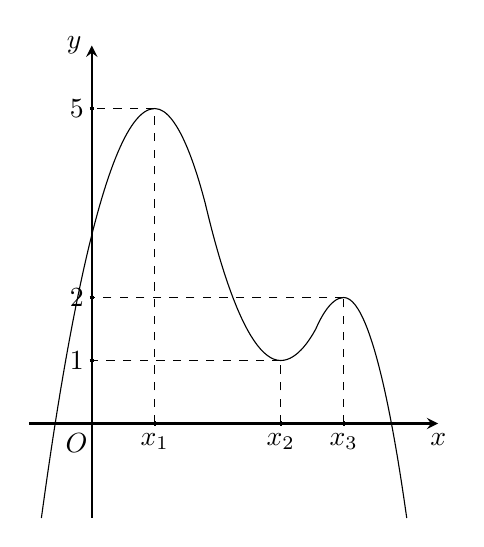
\begin{tikzpicture}[xscale=0.8,yscale=0.8,>=stealth]
			\draw[thick][->](-1,0)--(5.5,0)node[right,below]{$x$};
			\foreach \x in{1,3,4}\draw[xshift=\x cm,thick] (0pt,-1pt)--(0pt,1pt);
			\draw[thick][->](0,-1.5)--(0,6)node[above,left]{$y$};
			\foreach \y in {1,2,5}\draw[yshift=\y cm,thick] (-1pt,0pt)--(1pt,0pt)node[left]{$\y$};
			\draw(0,0) node[below left,xshift=2pt]{$O$};
			\draw(-0.8,-1.5) parabola bend (1,5)(1.8,3.5);
			\draw(1.8,3.5) parabola bend (3,1)(3.556,1.5);
			\draw(3.556,1.5) parabola bend (4,2)(5,-1.5);
			\draw[dashed](1,0)--(1,5) (1,5)--(0,5) (3,0)--(3,1) (3,1)--(0,1) (4,0)--(4,2) (4,2)--(0,2);
			\draw(1,0)node[below]{$x_1$} (3,0)node[below]{$x_2$} (4,0)node[below]{$x_3$};
	\end{tikzpicture}}
	\loigiai{
		Ta có $y'=f'(x)-\dfrac{2018}{2017}$.\\
		Khi đó $y'=0\Rightarrow f'(x)-\dfrac{2018}{2017}=0\Rightarrow f'(x)=\dfrac{2018}{2017}.$\\
		Dựa vào đồ thị ta thấy phương trình $f'(x)=0$ có $4$ nghiệm phân biệt. Do đó hàm số đã cho có $4$ điểm cực trị.
	}
\end{ex}
%Câu 18
\begin{ex}%[2D1K2-2]
	Cho hàm số bậc ba $y=ax^3+bx^2+cx+d$ có đồ thị nhận hai điểm $A(1;3)$ và $B(3;-1)$ làm hai điểm cực trị. Khi đó số điểm cực trị của đồ thị hàm số $y=\left|ax^2\big|x\big|+bx^2+c\big|x\big|+d\right|$ là
	\choice
	{$7$}
	{\True $11$}
	{$5$}
	{$9$}
	\loigiai{
		Xét hàm số $y=ax^3+bx^2+cx+d$ có $y'=3ax^2+2bx+c$. \\
		Theo giả thiết, ta có hệ phương trình $\left\{\begin{aligned}
			&y(1)=3 \\
			&y'(1)=0 \\
			&y(3)=-1 \\
			&y'(3)=0
		\end{aligned}\right. \Leftrightarrow \left\{\begin{aligned}
			&a+b+c+d=3 \\
			&3a+2b+c=0 \\
			&27a+9b+3c+d=-1 \\
			&27a+6b+c=0
		\end{aligned}\right. \Leftrightarrow \left\{\begin{aligned}
			&a=1 \\
			&b=-6 \\
			&c=9 \\
			&d=-1.
		\end{aligned}\right. $. \\
		Vậy hàm số đã cho là $y=f(x)=x^3-6x^2+9x-1$ có đồ thị $(C)$ như sau:
		\begin{center}
			\begin{tikzpicture}[>=stealth][scale=.6]
				\draw[->] (-1,0)--(4.5,0) node[below]{$x$};
				\draw[->] (0,-2.5)--(0,4.5) node[left]{$y$} ;
				\draw (0,0) node[below left]{$O$};
				\draw[samples=100, smooth, domain=-0.15:4.1] plot(\x,{(\x)^3-6*(\x)^2+9*(\x)-1}) node[left]{$(C)$};
			\end{tikzpicture}
		\end{center}
		Từ đồ thị $(C)$, ta suy ra đồ thị $(C_1)$ của hàm số $y={\big|x\big|}^3-6x^2+9\big|x\big|-1$ gồm có hai phần: \\
		+ Phần 1: Giữ nguyên phần đồ thị $(C)$ bên phải trục tung. \\
		+ Phần 2: Lấy đối xứng của phần 1 qua trục tung
		\begin{center}
			\begin{tikzpicture}[>=stealth][scale=.6]
				\draw[->] (-4.5,0)--(4.5,0) node[below]{$x$};
				\draw[->] (0,-1.5)--(0,4.5) node[left]{$y$} ;
				\draw (0,0) node[below left]{$O$};
				\draw[samples=100, smooth, domain=0:4.1] plot(\x,{(\x)^3-6*(\x)^2+9*(\x)-1}) node[left]{$(C_1$};
				\draw[samples=100, smooth, domain=-4.1:0] plot(\x,{-(\x)^3-6*(\x)^2-9*(\x)-1});
			\end{tikzpicture}
		\end{center}
		Từ đó suy ra đồ thị $(C_2)$ của hàm số $y=\left|{\big|x\big|}^3-6x^2+9\big|x\big|-1\right|$ gồm có hai phần: \\
		+ Phần 1: Giữ nguyên phần đồ thị $(C_1)$ phía trên trục hoành. \\
		+ Phần 2: Lấy đối xứng của phần đồ thị $(C_1)$ phía dưới trục hoành qua trục hoành.
		\begin{center}
			\begin{tikzpicture}[>=stealth][scale=.6]
				\draw[->] (-4.5,0)--(4.5,0) node[below]{$x$};
				\draw[->] (0,-1.5)--(0,4.5) node[left]{$y$} ;
				\draw (0,0) node[below left]{$O$};
				\draw[samples=100, smooth, domain=0.1206147584:2.347296355] plot(\x,{(\x)^3-6*(\x)^2+9*(\x)-1});
				\draw[samples=100, smooth, domain=3.532088886:4.1] plot(\x,{(\x)^3-6*(\x)^2+9*(\x)-1}) node[left]{$(C_2)$};
				\draw[samples=100, smooth, domain=-4.1:-3.532088886] plot(\x,{-(\x)^3-6*(\x)^2-9*(\x)-1});
				\draw[samples=100, smooth, domain=-2.347296355:-0.1206147584] plot(\x,{-(\x)^3-6*(\x)^2-9*(\x)-1});
				\draw[samples=100, smooth, domain=0:0.1206147584] plot(\x,{-(\x)^3+6*(\x)^2-9*(\x)+1});
				\draw[samples=100, smooth, domain=2.347296355:3.532088886] plot(\x,{-(\x)^3+6*(\x)^2-9*(\x)+1});
				\draw[samples=100, smooth, domain=-3.532088886:-2.347296355] plot(\x,{(\x)^3+6*(\x)^2+9*(\x)+1});
				\draw[samples=100, smooth, domain=-0.1206147584:0] plot(\x,{(\x)^3+6*(\x)^2+9*(\x)+1});
			\end{tikzpicture}
		\end{center}
		Do đó, đồ thị $(C_2)$ có $11$ điểm cực trị.}
\end{ex}
%Câu 19
\begin{ex}%[2D1K2-2]
	\immini {Cho hàm số bậc bốn $y=f(x)$. Biết rằng hàm số $y=f'(x)$ có đồ thị như hình vẽ bên. Hỏi hàm số  $y=f(5-x^2)$ có bao nhiêu điểm cực trị?
		\choice
		{$4$}
		{\True $7$}
		{$3$}
		{$9$}
	}
	{\begin{tikzpicture}[>=stealth,scale=0.4]
			\clip(-6,-4) rectangle (6.2,5.4);
			\draw[->] (-6,0)--(6,0);
			\draw[->] (0,-3)--(0,5);
			\draw (5.8,0) node[below] {$x$};
			\draw (0,5) node[left]{$y$};
			\draw (0,0) node[ below left]{$ O $};
			\draw[smooth,samples=300,domain=-4.5:5.1] plot(\x,{ (\x+4)*(\x-1)*(\x -4)*0.1});
			\draw (-4,0) node[below left] {$-4$};
			\draw (1,0) node[below] {$1$};
			\draw (4,0) node[below right] {$4$};
			\fill (0cm,0cm)circle (2pt);
			\fill (1cm,0cm) circle (2pt);
			\fill (4cm,0cm)circle (2pt);
			\fill (-4cm,0cm) circle (2pt);
	\end{tikzpicture}}
	\loigiai
	{ Xét hàm số  $y=f(5-x^2)$, ta có $$y'=-2x\cdot f'(5-x^2)\Rightarrow y'=0 \Leftrightarrow \hoac{&x=0\\&5-x^2=-4\\&5-x^2=1\\&5-x^2=4}\Leftrightarrow \hoac {&x=0\\&x^2=9\\&x^2=4\\&x^2=1}\Leftrightarrow \hoac {&x=0\\&x=\pm 3\\&x=\pm 2\\&x=\pm 1.}$$\\ Do đó hàm số $y=f(5-x^2)$ có $7$ điểm cực trị.
	}
\end{ex}
%Câu 20
\begin{ex}%[2D1K2-2]
	Cho hàm số $y=f(x)$ có bảng biến thiên như sau
	\begin{center}
		
\begin{tikzpicture}
			\tkzTabInit[lgt=1.5,espcl=2]{$x$/1,$f’(x)$/1,$f(x)$/2}{$-\infty$,$-1$,$3$,$+\infty$}%
			\tkzTabLine{,+,z,-,z,+,}%
			\tkzTabVar{-/$-\infty$ , +/$5$,-/$1$, +/$+\infty$}%
		\end{tikzpicture}
	\end{center}
	Đồ thị hàm số $y=\left|f(x)\right|$ có bao nhiêu điểm cực trị?
	\choice
	{$2$}
	{$5$}
	{\True $3$}
	{$4$}
	\loigiai{
		Ta có $y=\left|f(x)\right|=\heva{&f(x),&\text{ nếu } f(x)\geq 0\\&-f(x), &\text{ nếu } f(x)<0}$.\\
		Suy ra bảng biến thiên của hàm số $y=\left|f(x)\right|$ có dạng:
		\begin{center}
			
\begin{tikzpicture}
				\tkzTabInit[lgt=1.5,espcl=2]{$x$/1,$y'$/1,$y$/2}{$-\infty$,$x_0$,$-1$,$3$,$+\infty$}%
				\tkzTabLine{,-,t,+,z,-,z,+,}%
				\tkzTabVar{+/$+\infty$,-/$0$ , +/$5$,-/$1$, +/$+\infty$}%
			\end{tikzpicture}
		\end{center}
		Do đó đồ thị hàm số $y=\left|f(x)\right|$ có $3$ điểm cực trị.
	}
\end{ex}
%Câu 21
\begin{ex}%[2D1K2-2]
	\immini{Cho hàm số bậc bốn $y=f(x)$ có đồ thị như hình vẽ bên. Hỏi đồ thị hàm số $y=\left|f(x)\right|$ có bao
		nhiêu điểm cực trị?
		\choice
		{\True $5$}
		{$3$}
		{$4$}
		{$2$}
	}
	{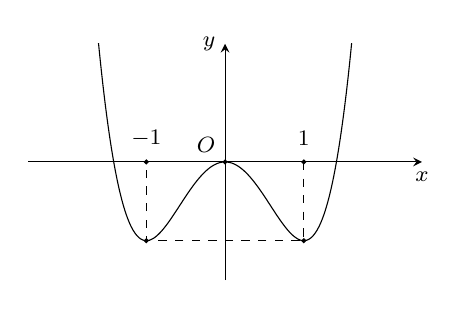
\begin{tikzpicture}[scale=1,>=stealth,font=\footnotesize]
			\def\mx{-2.5} \def\max{2.5}
			\def\my{-1.5} \def\may{1.5}
			\def\hamso(#1,#2){plot [samples=200,smooth,domain=#1:#2](\x,{
					1*(\x)^4-2*(\x)^2
				})}
			\foreach \p in {-1,1}{
				\draw[fill=black] (\p,0)circle (.7pt) node[shift={(90:.3)}]{$\p$};
				\draw[fill=black] (\p,-1)circle (.7pt);}
			\draw[fill=black] (0,0)circle (.7pt)node [above left] {$O$};
			\draw[dashed,thin] (1,0)|-(0,-1)-|(-1,0);
			%===========================================
			\draw[->] (\mx,0)--(\max,0) node[below] {$x$};
			\draw[->] (0,\my)--(0,\may) node[left] {$y$};
			\clip (\mx,\my) rectangle (\max,\may);
			\draw \hamso(\mx,\max);
	\end{tikzpicture}}
	\loigiai{
		Đồ thị hàm số $y=\left|f(x)\right|$.
		\begin{center}
			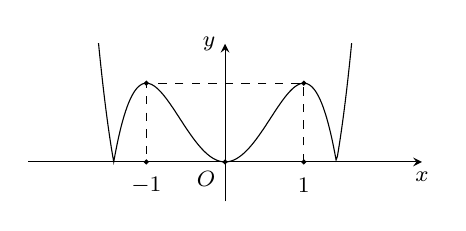
\begin{tikzpicture}[scale=1,>=stealth,font=\footnotesize]
				\def\mx{-2.5} \def\max{2.5}
				\def\my{-0.5} \def\may{1.5}
				\def\f(#1){
					abs(1*(#1)^4-2*(#1)^2
					)}
				\foreach \p in {-1,1}{
					\draw[fill=black] (\p,0)circle (.7pt) node[shift={(-90:.3)}]{$\p$};
					\draw[fill=black] (\p,1)circle (.7pt);}
				\draw[fill=black] (0,0)circle (.7pt)node [below left] {$O$};
				\draw[dashed,thin] (1,0)|-(0,1)-|(-1,0);
				%===========================================
				\draw[->] (\mx,0)--(\max,0) node[below] {$x$};
				\draw[->] (0,\my)--(0,\may) node[left] {$y$};
				\clip (\mx,\my) rectangle (\max,\may);
				\draw[samples=300] plot[domain=\mx:\max] (\x,{\f(\x)});
			\end{tikzpicture}
		\end{center}
		Suy ra đồ thị hàm số $y=\left|f(x)\right|$ có $5$ cực trị.
	}
\end{ex}
\Closesolutionfile{ans}
\subsection{Bảng đáp án}
\inputansbox{8}{ans/ANS-DANG-19}

